% ---------------------------------------------------------------------------
%  Final project report, IEEE conference format.
%
%  Compile with pdfLaTeX (Overleaf: "pdfLaTeX" or the default IEEEtran recipe).
%  No external files and no images are required: every figure is drawn with
%  TikZ/pgfplots from the numbers in results/.
%
%  Before submitting, replace the institution placeholder in the author block.
% ---------------------------------------------------------------------------
\documentclass[conference]{IEEEtran}

\usepackage[T1]{fontenc}
\usepackage[utf8]{inputenc}
\usepackage[table]{xcolor}
\usepackage{booktabs}
\usepackage{graphicx}
\usepackage{array}
\usepackage{tikz}
\usetikzlibrary{positioning,arrows.meta,patterns,calc}
\usepackage{pgfplots}
\pgfplotsset{compat=1.18}
\usepgfplotslibrary{groupplots}
\usepackage{url}

% ---------------------------------------------------------------------------
%  Palette. One hue per mechanism, used consistently in every figure and table:
%    purple = client, outside the server
%    blue   = network ingestion / lock-free path / SPSC
%    orange = queue hand-off / blocking mutex path
%    green  = book data structure and allocator
%    teal   = sinks and recording
%    red    = the tail, collapse, failure
% ---------------------------------------------------------------------------
\definecolor{cblue}{HTML}{1F4E79}
\definecolor{cblueL}{HTML}{E9F1F9}
\definecolor{corange}{HTML}{B45309}
\definecolor{corangeL}{HTML}{FDF2E6}
\definecolor{cgreen}{HTML}{2F6B3A}
\definecolor{cgreenL}{HTML}{EAF4EB}
\definecolor{cpurple}{HTML}{5B3E86}
\definecolor{cpurpleL}{HTML}{F0EBF8}
\definecolor{cteal}{HTML}{0F6E6E}
\definecolor{ctealL}{HTML}{E4F3F3}
\definecolor{cred}{HTML}{A2261E}
\definecolor{credL}{HTML}{FBEBE9}
\definecolor{cgray}{HTML}{555555}
\definecolor{cgrayL}{HTML}{F2F2F2}

% Take-away line after a table or figure: coloured rule, italic text.
\newcommand{\reading}[1]{%
  \par\vspace{1pt}\noindent
  \textcolor{corange}{\rule[-0.2ex]{2.2pt}{1.05em}}\hspace{3pt}%
  \textit{\textcolor{cgray}{#1}}\par\vspace{2pt}}

% Plots: light grid, coloured series, no chart junk.
\pgfplotsset{
  every axis/.append style={
    font=\scriptsize,
    label style={font=\scriptsize},
    tick label style={font=\scriptsize},
    legend style={font=\scriptsize, draw=none, fill=none},
    grid=major,
    grid style={cblue!10},
    axis line style={black!65},
    tick style={black!55},
    every axis title/.append style={font=\scriptsize\bfseries, color=cblue},
  },
}

% Units. Written as math so they render identically in every engine.
\newcommand{\us}{\,$\mu$s}
\newcommand{\ns}{\,ns}
\newcommand{\Mops}{\,M\,orders/s}

\begin{document}

\title{Design, Benchmarking, and Tail-Latency Analysis of a High-Performance
Order-Book Matching Engine}

\author{%
\IEEEauthorblockN{Piyush Satiya, Prayag Kirar, Sanskar Sharma, Sorabh Baldeva,
and Ved Gupta}
\IEEEauthorblockA{Department of Computer Science and Engineering\\
Indian Institute of Information Technology\\
Gandhinagar, Gujarat\\
Roll Nos.: 202451130, 202451134, 202451148, 202451156, 202451166}
}

\maketitle

\begin{abstract}
We measure where latency and tail latency are actually spent in a two-thread
producer--consumer pipeline: a TCP network thread feeding a single-threaded
price--time-priority matching engine through either a mutex ring buffer or a
lock-free single-producer/single-consumer (SPSC) ring buffer, behind either
\texttt{epoll} or \texttt{io\_uring}, with the order book implemented twice.
Every order is timestamped twice inside the server, so latency is attributed to
an arrival component (client send to parse) and a service component (parse to
match), and every run reports both threads' accumulated run-queue wait from
\texttt{schedstat}. Across 231 recorded runs, median latency at 200\,000
orders/s is about 25\us{} of which the matching step is about 3\us: 86--88\% of
typical latency is ingress and wake-up, not matching. The two queues are
statistically indistinguishable at the median ($p=0.15$) but differ by
$1.8\times$ at p99 and $3.3\times$ in the matching-side p99.9, and by
$1.75\times$ in throughput (5.86 versus 3.34\Mops). At 6.4\Mops{} offered, the
SPSC path absorbed the load with zero full-queue waits, while the mutex path
collapsed to 3.3\Mops{} in two of three runs. The book design matters more than
the queue at moderate load ($2.9\times$ throughput; a 10.97\,ms worst case
reduced to 26.7\us), whereas the slab allocator's isolated
$1.36$--$1.57\times$ advantage is not resolvable end-to-end ($p=0.37$). Pinning
the engine cut its run-queue wait tenfold without a significant end-to-end
effect ($p=0.14$), and a controlled confinement experiment shows that
millisecond-scale outliers are host ingress delay: 2.40\,ms to 142\us{} p99.9
with no code change.
\end{abstract}

\begin{IEEEkeywords}
high-performance computing, producer--consumer, tail latency, lock-free queues,
false sharing, CPU affinity, epoll, io\_uring, performance measurement
\end{IEEEkeywords}

\section{Introduction}

A large class of systems has one shape: several producers, a bounded queue, and
a single thread that owns all mutable state. Telemetry collectors, packet
processors, log shippers and exchange gateways differ in payload but not in
structure, and in all of them the state-owning thread is cheap compared with the
machinery that delivers work to it. An order book makes this shape concrete and
falsifiable: price--time priority is deterministic, every configuration must
produce identical output, and the matching work is small enough that anything
interesting in the latency distribution must come from the operating system.

This is therefore an operating-systems study, not a finance study. The matching
logic is deliberately single-threaded; the experiment changes one OS mechanism
at a time---synchronization, memory allocation, CPU scheduling and I/O---and
asks whether the resulting change in latency can be explained by a mechanism
rather than by folklore. The question the project set out to answer is:

\begin{quote}
\itshape What happens to latency and tail latency when synchronization, memory
allocation, CPU scheduling and I/O are changed one at a time, and can the result
be explained from OS mechanisms rather than from folklore?
\end{quote}

\subsection{Contributions}
\begin{itemize}
\item An instrumented pipeline that timestamps every order twice inside the
server and reads per-thread run-queue wait from
\texttt{/proc/thread-self/schedstat}, so arrival delay and service delay are
separated per run rather than inferred.
\item A single-variable measurement matrix---queue $\times$ scheduling $\times$
network, plus book and allocator variants---of 231 recorded runs, gated by a
clean-run criterion and analysed with permutation tests on medians.
\item Component microbenchmarks that bracket the integrated numbers and isolate
queue hand-off, book data structure, allocator and cache-line layout
individually.
\item A saturation sweep and a controlled host-confinement experiment, which
expose two failure modes that a fixed-offered-rate benchmark cannot see: a
bistable blocking queue, and millisecond ingress delays caused by an unrelated
process.
\end{itemize}

\subsection{Summary of Results}
The matching step costs about 94\ns; the pipeline without a network costs
299\ns{} at the median; the complete TCP pipeline costs about 25\us{} at the
median and 86\us{} at p99.9. Consequently the queue is invisible at the median
and decisive in the tail, the book data structure dominates the worst case, the
slab allocator is measurable only in isolation, and pinning without isolation
moves a counter without moving the distribution. Section~\ref{sec:results}
quantifies each of these; Section~\ref{sec:discussion} relates them to the
central question.

\section{System Design}
\label{sec:design}

\subsection{Architecture}
Fig.~\ref{fig:arch} shows the system as built. A client sends fixed 40-byte
little-endian messages over TCP with \texttt{TCP\_NODELAY}, each carrying a
\texttt{CLOCK\_MONOTONIC} send timestamp. The network thread parses messages,
stamps each order and pushes it into the queue; the engine thread pops orders,
matches or rests them, and reports trades to a counting sink that accumulates
trade count, traded quantity and notional. Those three numbers are the
correctness checksum: identical seeds must produce identical values in every
configuration.

Every stage in the figure is an interface with exactly two implementations
(dashed), and every experiment changes one of them at a time while the others
are held fixed. The matching loop itself is a single template,
\texttt{MatchingEngine<Book,Sink>}, so swapping the book cannot change the
matching logic; the network backends push orders through the same function
pointer, so the queue cannot tell \texttt{epoll} from \texttt{io\_uring}. That
is what makes the comparisons in Section~\ref{sec:results} single-variable.

\begin{figure*}[!t]
\centering
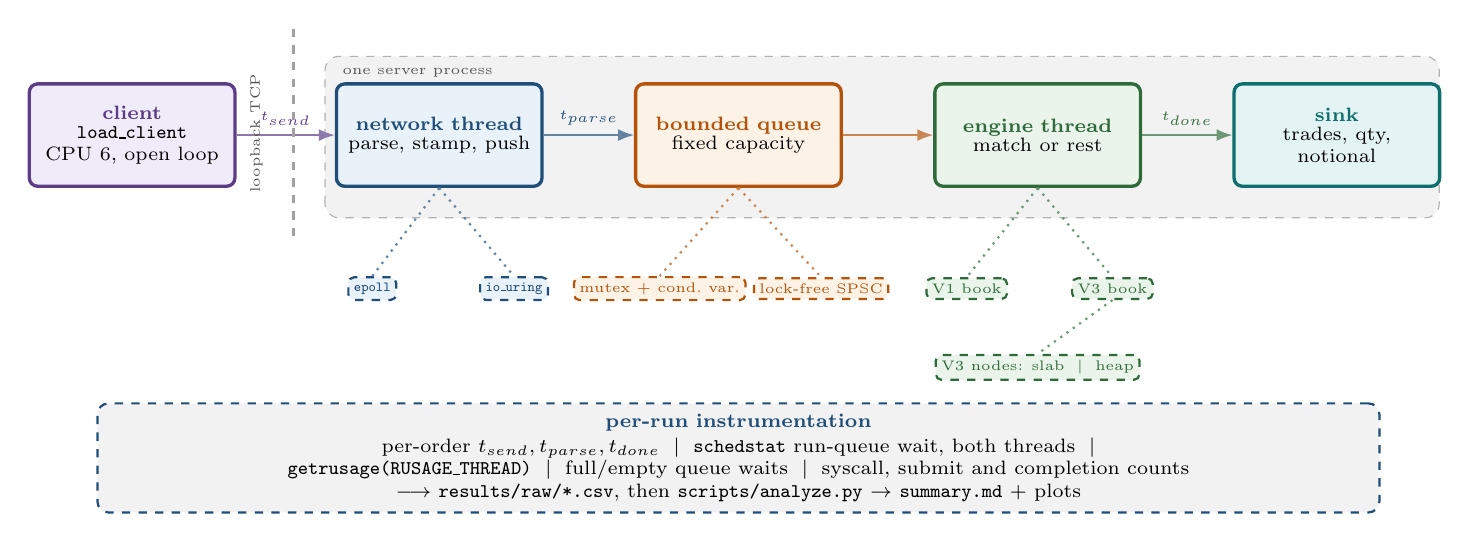
\begin{tikzpicture}[font=\scriptsize, >=Latex,
  stage/.style={draw, very thick, rounded corners=3pt, align=center,
                inner sep=3pt, minimum height=13mm, text width=24mm},
  variant/.style={draw, thick, dashed, rounded corners=2pt, align=center,
                  inner sep=2pt, font=\tiny, fill=white},
  flow/.style={->, semithick, black!65},
  stamp/.style={font=\tiny\bfseries}]

% ---- server process panel -------------------------------------------------
\fill[cgrayL, rounded corners=5pt] (2.45,-1.05) rectangle (16.6,1.0);
\draw[cgray!45, dashed, rounded corners=5pt] (2.45,-1.05) rectangle (16.6,1.0);
\node[font=\tiny, cgray, anchor=north west] at (2.55,0.97) {one server process};

% ---- main data path -------------------------------------------------------
\node[stage, draw=cpurple, fill=cpurpleL] (c) at (0,0)
  {\textcolor{cpurple}{\textbf{client}}\\[-1pt]
   \texttt{load\_client}\\ CPU 6, open loop};
\node[stage, draw=cblue, fill=cblueL] (n) at (3.9,0)
  {\textcolor{cblue}{\textbf{network thread}}\\[-1pt]
   parse, stamp, push};
\node[stage, draw=corange, fill=corangeL] (q) at (7.7,0)
  {\textcolor{corange}{\textbf{bounded queue}}\\[-1pt]
   fixed capacity};
\node[stage, draw=cgreen, fill=cgreenL] (e) at (11.5,0)
  {\textcolor{cgreen}{\textbf{engine thread}}\\[-1pt]
   match or rest};
\node[stage, draw=cteal, fill=ctealL] (s) at (15.3,0)
  {\textcolor{cteal}{\textbf{sink}}\\[-1pt]
   trades, qty, notional};

\draw[flow, draw=cpurple!70] (c) -- node[above, stamp, text=cpurple] {$t_{\text{send}}$} (n);
\draw[flow, draw=cblue!70]   (n) -- node[above, stamp, text=cblue]   {$t_{\text{parse}}$} (q);
\draw[flow, draw=corange!70] (q) -- (e);
\draw[flow, draw=cgreen!70]  (e) -- node[above, stamp, text=cgreen]  {$t_{\text{done}}$} (s);

% process boundary between client and server
\draw[dashed, cgray!55, thick] (2.05,1.35) -- (2.05,-1.35);
\node[font=\tiny, cgray, rotate=90, anchor=south] at (1.78,0.02) {loopback TCP};

% ---- swap-in implementations ---------------------------------------------
\node[variant, draw=cblue,   fill=cblueL,   text=cblue]   (ep) at (3.05,-1.95) {\texttt{epoll}};
\node[variant, draw=cblue,   fill=cblueL,   text=cblue]   (ur) at (4.85,-1.95) {\texttt{io\_uring}};
\node[variant, draw=corange, fill=corangeL, text=corange] (mu) at (6.7,-1.95)  {mutex + cond.\ var.};
\node[variant, draw=corange, fill=corangeL, text=corange] (sp) at (8.75,-1.95) {lock-free SPSC};
\node[variant, draw=cgreen,  fill=cgreenL,  text=cgreen]  (v1) at (10.6,-1.95) {V1 book};
\node[variant, draw=cgreen,  fill=cgreenL,  text=cgreen]  (v3) at (12.45,-1.95){V3 book};

\foreach \src/\dst/\col in {n/ep/cblue, n/ur/cblue, q/mu/corange,
                            q/sp/corange, e/v1/cgreen, e/v3/cgreen}
  \draw[dotted, thick, \col!70] (\src.south) -- (\dst.north);

\node[variant, draw=cgreen, fill=cgreenL, text=cgreen] (al) at (11.5,-2.95)
  {V3 nodes: slab $\;\mid\;$ heap};
\draw[dotted, thick, cgreen!70] (v3.south) -- (al.north);

% ---- instrumentation ------------------------------------------------------
\node[draw=cblue, thick, dashed, rounded corners=4pt, align=center,
      inner sep=4pt, text width=160mm, fill=cgrayL] (i) at (7.7,-4.1)
  {\textcolor{cblue}{\textbf{per-run instrumentation}}\\[1pt]
   per-order $t_{\text{send}},t_{\text{parse}},t_{\text{done}}$
   \;\textbar\; \texttt{schedstat} run-queue wait, both threads
   \;\textbar\; \texttt{getrusage(RUSAGE\_THREAD)}
   \;\textbar\; full/empty queue waits
   \;\textbar\; syscall, submit and completion counts\\
   $\longrightarrow$ \texttt{results/raw/*.csv}, then
   \texttt{scripts/analyze.py} $\rightarrow$ \texttt{summary.md} + plots};

\end{tikzpicture}
\caption{Architecture as built, one colour per mechanism: purple client, blue
network ingestion, orange queue, green book, teal sink. Each server-side stage
has exactly two interchangeable implementations (dashed chips), and each
experiment swaps one of them while holding the rest fixed, which is what makes
the comparisons in Section~\ref{sec:results} single-variable. Each order is
stamped at the client ($t_{\text{send}}$), at parse time in the network thread
($t_{\text{parse}}$) and at completion on the engine thread
($t_{\text{done}}$), so arrival latency $t_{\text{parse}}-t_{\text{send}}$ and
service latency $t_{\text{done}}-t_{\text{parse}}$ are both measured inside the
server, with no clock synchronisation. The grey band is the instrumentation
that turns a run into every table and plot in Section~\ref{sec:results}.}
\label{fig:arch}
\end{figure*}

\subsection{Order Books}
\texttt{MatchingEngine<Book,Sink>} is a template over the book and the sink, so
the matching logic is identical for both implementations and cannot drift.

\textbf{V1 (reference).} \texttt{std::map<Price,std::list<Order>>} per side plus
an \texttt{std::unordered\_map<OrderId,iterator>} for cancels. It is correct,
simple, and the baseline that makes the optimized version's gains attributable.

\textbf{V3 (optimized).} Prices index a flat array
(\texttt{levels\_[price-min\_price]}), so locating a level is an addition rather
than a tree walk. Each level is an intrusive doubly linked list of nodes that are
\texttt{alignas(64)}, and a 48-byte order plus two pointers is exactly one
64-byte cache line (\texttt{static\_assert(sizeof(Node)==64)}). Best price is
found with a two-level bitmap and \texttt{ctz}/\texttt{clz}; empty-level
transitions update the bitmap incrementally. An open-addressing table, sized at
construction never to rehash, maps order id to node. The trade-offs are explicit:
prices must fall in a fixed window and capacity is fixed, both checked and
counted.

\subsection{Synchronization}
\textbf{Mutex ring buffer.} A fixed circular array guarded by
\texttt{std::mutex} with \texttt{not\_full} and \texttt{not\_empty} condition
variables. This is the ``OS does the scheduling'' baseline: every
empty-to-nonempty transition requires a wakeup.

\textbf{SPSC ring buffer.} One producer writes \texttt{tail\_}, one consumer
writes \texttt{head\_}, so no variable is written by both threads and no CAS loop
is needed~\cite{lamport,michael}. The indices occupy separate cache lines
(\texttt{alignas(64)}); each side caches the peer index locally and re-reads the
shared atomic only when the queue looks full or empty; counters increase
monotonically so full/empty is a subtraction and no slot is wasted, with the slot
address computed as \texttt{counter \& mask}. Ordering is the minimum required:
the producer stores the slot and publishes with \texttt{release}, the consumer
loads with \texttt{acquire} before reading it, and symmetrically on the return
path~\cite{boehm}. Waiting is a bounded spin with \texttt{\_\_builtin\_pause},
followed by a \texttt{yield} once per 4096 spins; yielding on every failed
iteration degenerates into a \texttt{sched\_yield} storm. The yield count is
exported so busy-wait cost is visible in the results.

\subsection{Allocation}
\texttt{SlabAllocator<T,N>} pre-allocates one block, carves it into
\texttt{sizeof(T)} chunks, and threads free slots through a free list stored in
the slots themselves, so bookkeeping costs no extra memory.
\texttt{HeapAllocator} is the control: identical book code, but each node comes
from aligned \texttt{operator new}/\texttt{delete}.

\subsection{Scheduling and Affinity}
In \texttt{pin} mode only the engine is pinned (CPU 2) via
\texttt{pthread\_setaffinity\_np}; the network thread is deliberately left
floating. The environment variable \texttt{ME\_PIN\_NET=1} additionally pins the
network thread (CPU 4), which we use only as a probe. In \texttt{rt} mode the
engine requests \texttt{SCHED\_FIFO} at priority 50; on this host the call fails
with \texttt{EPERM} (\texttt{rtprio\_limit=0}, no \texttt{CAP\_SYS\_NICE}), and
the failure is recorded rather than silently downgraded. The client is pinned to
CPU 6 so that client jitter is not mistaken for server jitter; a probe removes
that pinning.

\subsection{Network Ingestion}
Both backends implement the same \texttt{INetworkServer} interface and push
through the same function pointer, so the queue and engine cannot tell them
apart. \texttt{epoll} waits on a listening and a connected descriptor and then
runs an edge-triggered drain loop of \texttt{recv()} until \texttt{EAGAIN};
\texttt{io\_uring} keeps one single-shot receive in flight and re-posts it after
each completion~\cite{axboe}. Both use a 4096-byte per-connection buffer that
carries partial messages across reads, and both parse with the same routine.

\section{Methodology}
\label{sec:method}

\subsection{Workload and Protocol}
One TCP client with a deterministic seed (42) drives the server. Latency runs
use an \emph{open loop} at 200\,000 orders/s in 64-order batches: the client
paces itself, so a slow server cannot slow the sender. Each run sends
1\,010\,000 orders and discards the first 10\,000 as warm-up; ten repetitions per
configuration are summarised by their median, and every raw run is retained.
Throughput runs use the same client unthrottled (1024-order batches,
2\,000\,000 orders, five repetitions). Saturation runs fix an offered rate,
measure a two-second window (shortened at high rates to stay inside the
4-million-sample recorder) and count blocking \texttt{push}/\texttt{pop} calls;
these are the only runs that exercise a full queue. In total the matrix records
231 pipeline runs (120 integrated, 45 allocator-in-pipeline, 54 saturation,
12 probe) plus 36 component repetitions. Every comparison below changes exactly
one of the stages or swap points in Fig.~\ref{fig:arch}.

\subsection{Instrumentation}
Three in-process sources replace the profiler we did not have:

\begin{itemize}
\item \textbf{Two timestamps per order, one from each side.} \texttt{enqueue\_time}
is taken on the network thread after parsing, so arrival and service latency are
separated without clock synchronisation. Adding the field kept the book node at
exactly 64 bytes, so the measurement did not change the structure it measures.
\item \textbf{\texttt{schedstat}.} The second field of
\texttt{/proc/thread-self/schedstat} is the cumulative time a thread spent
runnable but off-CPU. Reading it for both threads at the end of a run converts
``the scheduler probably interfered'' into a number.
\item \textbf{Counter columns.} \texttt{getrusage(RUSAGE\_THREAD)} supplies
voluntary and involuntary context switches and CPU time; the backends count
waits, receives, submits and completions; the queues count full and empty waits.
\end{itemize}

A run is \emph{clean} if no order was already more than 1\,ms old when the
network thread parsed it. Contaminated runs are recorded and listed rather than
deleted, so the matrix stays auditable; configurations are ranked on clean runs
only, and a configuration with no clean run is reported as not measurable on
this host instead of being used as evidence about the code. Percentiles are used
throughout because an average can look excellent while hiding a 10\,ms stall,
and every effect in this paper is a tail effect~\cite{gregg}.

\subsection{Host Conditions}
Table~\ref{tab:conditions} lists the environment. Two details matter for
interpretation. First, the platform profile is fixed at \texttt{performance}
with the energy-performance preference set to \texttt{performance} on all twelve
CPUs, but \texttt{intel\_pstate} still owns the frequency, so clocks move
between 0.8 and 4.4\,GHz. Second, a five-second sampler recorded package
temperature and P-core frequency for the whole session (199 samples):
47--71\,$^\circ$C, median P-core frequency 4.37\,GHz, no sample at or above
95\,$^\circ$C, and no sample below 4.0\,GHz except between runs or during the
single-threaded book benchmark. There was no thermal throttling, so the order in
which configurations ran does not bias comparisons through a drifting clock.

\begin{table}[!t]
\centering
\caption{Measurement conditions.}
\label{tab:conditions}
\small
\setlength{\tabcolsep}{4pt}
\begin{tabular}{@{}ll@{}}
\arrayrulecolor{cblue}\toprule
\rowcolor{cblueL}\textbf{Item} & \textbf{Value} \\
\arrayrulecolor{black!25}\midrule
Kernel      & \texttt{7.2.9-arch1-1}, \texttt{PREEMPT\_DYNAMIC} \\
CPU         & 4 P-cores $\times$ 2 SMT ($\le$4.4\,GHz) \\
            & + 4 E-cores ($\le$3.1\,GHz), 12 threads \\
Compiler    & GCC 16.2.1, \texttt{-O3 -DNDEBUG} \\
liburing    & 2.15 \\
Session     & TTY login, no graphical session \\
Load average at start & 0.21 / 0.05 / 0.02 \\
Platform profile & \texttt{performance}, EPP \texttt{performance} \\
Governor    & \texttt{powersave}, turbo on, SMT on \\
\texttt{SCHED\_FIFO} & denied (\texttt{EPERM}) \\
\texttt{perf}, \texttt{strace} & unavailable \\
\texttt{isolcpus}, \texttt{nohz\_full} & unavailable (root) \\
Package temperature & 47--71\,$^\circ$C \\
P-core frequency & median 4.37\,GHz, max 4.42\,GHz \\
\arrayrulecolor{cblue}\bottomrule
\end{tabular}
\end{table}

\subsection{Statistics}
Differences are tested with a two-sided permutation test on the difference of
medians, clean runs only. At these sample sizes every label assignment can be
enumerated, so the test is exact ($\binom{20}{10}=184\,756$ splits for a
ten-versus-ten comparison, $\binom{19}{9}=92\,378$ for nine-versus-ten) and the
reported $p$ values carry no resampling error. With $n=9$--10 per configuration
this resolves differences of roughly 30\% or more; anything smaller is reported
as not distinguishable. Claims that rest on fewer runs are labelled as such.

\subsection{Reproducibility}
One command (\texttt{scripts/run\_session.sh}) captures the environment, rebuilds
in Release, runs all five measurement phases, runs both analysers and samples
thermal state; it refuses to start on a dirty tree and preserves the previous
session's data. The generated tables quoted here are
\texttt{results/summary.md} and \texttt{results/components-summary.md}; the
environment record is \texttt{results/env.txt}. The test suite (7 tests,
including differential book tests and a wire-format parser) passes in Release and
under AddressSanitizer/UBSan, and the SPSC ring buffer passes under
ThreadSanitizer. \texttt{scripts/verify.sh} additionally checks that
\texttt{epoll} and \texttt{io\_uring} agree on trades, quantity and notional.

\section{Results}
\label{sec:results}

All latency figures are client send to engine completion on the same host, in
microseconds unless stated, and are medians across repetitions. ``Clean'' counts
runs that passed the ingress gate of Section~\ref{sec:method}. The section asks
one question at a time: a table carries the numbers, a figure carries the shape,
and the italic line after it states the answer.

\subsection{Component Floors}
Table~\ref{tab:components} brackets the integrated pipeline from below. Two
observations set up everything that follows.

\textbf{The book is a tail problem, not a mean problem.} V3 delivers
$2.9\times$ the throughput of V1 but is \emph{slower} at the median (94 versus
81\ns). Its value is that the worst case falls from 10.97\,ms to 26.7\us---a
factor of 411. Both books produce identical trade counts (1\,093\,640 trades),
so the difference is not matching less.

\textbf{The queue is a hand-off problem.} With no network involved and the same
book, replacing the mutex with the SPSC ring cuts p50 from 1.6\us{} to 299\ns{}
($5.4\times$) and raises throughput $2.1\times$ (7.35 versus 3.49\Mops). All four
combinations agree on 789\,497 trades and 20\,135\,763 traded quantity.

\begin{table*}[!t]
\centering
\caption{Component floors: single-threaded book (top, green) and two-thread
queue plus book with no network (bottom, teal). Latencies in $\mu$s; medians of
9 repetitions. Red marks the worst tail in each block.}
\label{tab:components}
\small
\setlength{\tabcolsep}{6pt}
\begin{tabular}{@{}lrrrrr@{}}
\arrayrulecolor{cblue}\toprule
\rowcolor{cblueL}\textbf{Variant} & \textbf{Throughput} & \textbf{p50} & \textbf{p99} & \textbf{p99.9} & \textbf{max} \\
\arrayrulecolor{cblue!45}\midrule
\rowcolor{cgreenL}\multicolumn{6}{@{}l}{\textcolor{cgreen}{\emph{Single-threaded book, 2\,M mixed operations}}} \\
V1\ \ \texttt{map}+\texttt{list}+\texttt{unordered\_map} & 11.63\Mops & \textbf{0.081} & 0.420 & 0.595 & \textcolor{cred}{\textbf{10\,970}} \\
V3\ \ array + slab + bitmap & \textbf{33.68\Mops} & 0.094 & \textbf{0.247} & \textbf{0.374} & \textbf{26.7} \\
\arrayrulecolor{cblue!45}\midrule
\rowcolor{ctealL}\multicolumn{6}{@{}l}{\textcolor{cteal}{\emph{Queue + book, 1.01\,M orders at 200k orders/s}}} \\
SPSC + V3 & \textbf{7.35\Mops} & \textbf{0.299} & \textbf{1.6} & \textbf{13.2} & \textbf{160} \\
SPSC + V1 & 5.77\Mops & 0.247 & 0.836 & \textcolor{cred}{5\,400} & \textcolor{cred}{10\,240} \\
mutex + V3 & 3.49\Mops & 1.6 & 3.9 & 14.6 & 404 \\
mutex + V1 & 3.27\Mops & 1.6 & 3.6 & \textcolor{cred}{6\,260} & \textcolor{cred}{11\,020} \\
\arrayrulecolor{cblue}\bottomrule
\end{tabular}
\end{table*}

\reading{Microbenchmarks bound the pipeline from below: the book is 94\ns{} of
work, and the queue hand-off is the only thing that moves the median once the
network is out of the picture.}

\subsection{Integrated Latency}
Table~\ref{tab:latency} is the main result. Every configuration sits between
24 and 29\us{} at the median: the spread across queue, network and scheduler
choices is smaller than the distance from any median to the same row's p95. The
distributions, however, are not the same shape. SPSC climbs about 3\us{} between
p95 and p99; the mutex climbs about 30\us{} between p50 and p95. Two
distributions with the same centre and different bodies.

Fig.~\ref{fig:quantiles} draws that difference with the probability axis
stretched near 100\%, so the tail occupies the upper half of the plot. The four
curves separate not at the median but between p90 and p99.9: the queue is a
median-neutral, tail-relevant choice.

\begin{figure}[!t]
\centering
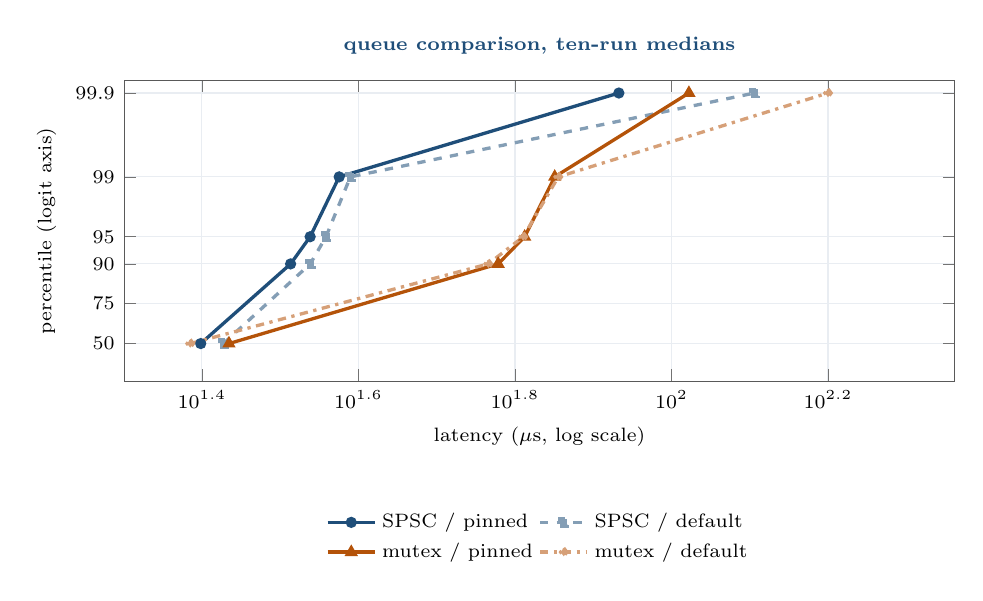
\begin{tikzpicture}
\begin{axis}[
  width=\columnwidth, height=5.4cm,
  xmode=log, xmin=20, xmax=230,
  ymin=-0.45, ymax=3.15,
  ytick={-0.4771,0,0.4771,0.9542,1.2788,1.9956,3},
  yticklabels={25,50,75,90,95,99,99.9},
  xlabel={latency ($\mu$s, log scale)},
  ylabel={percentile (logit axis)},
  legend cell align=left,
  legend style={at={(0.5,-0.40)}, anchor=north, legend columns=2, draw=none},
  title={queue comparison, ten-run medians},
]
\addplot[cblue, very thick, mark=*, mark size=1.4pt] coordinates {
  (25.03,0.000) (32.61,0.954) (34.54,1.279) (37.62,1.996) (85.65,3.000)};
\addplot[cblue!55, very thick, dashed, mark=square*, mark size=1.3pt] coordinates {
  (26.76,0.000) (34.55,0.954) (36.19,1.279) (38.88,1.996) (127.68,3.000)};
\addplot[corange, very thick, mark=triangle*, mark size=1.6pt] coordinates {
  (27.20,0.000) (60.05,0.954) (64.92,1.279) (70.93,1.996) (105.25,3.000)};
\addplot[corange!55, very thick, dashdotted, mark=diamond*, mark size=1.5pt] coordinates {
  (24.27,0.000) (58.33,0.954) (64.66,1.279) (71.67,1.996) (158.47,3.000)};
\legend{SPSC / pinned, SPSC / default, mutex / pinned, mutex / default}
\end{axis}
\end{tikzpicture}
\caption{Latency quantiles at 200\,000 orders/s, all four queue/scheduler
combinations with \texttt{epoll}; blue is the lock-free queue, orange the
blocking one. Each curve uses the ten-run medians of Table~\ref{tab:latency}, so
the marker at 99.9\% is that table's p99.9 column. The medians are within 3\us{}
of each other while the matched p99 values differ by $1.8\times$ and the p99.9
values by $1.2\times$.}
\label{fig:quantiles}
\end{figure}

120 of 122 latency runs were clean. The two exceptions are single startup
episodes, recorded with their order counts: 64 orders in the first run of the
first configuration (maximum arrival 2.17\,ms with the network thread's run-queue
wait at 0.0\,ms, i.e.\ the client was descheduled before \texttt{send}) and 192
orders in one probe run.

\begin{table*}[!t]
\centering
\caption{Integrated latency at 200\,000 orders/s, $n=10$ per configuration.
Latencies in $\mu$s. Blue rows use the lock-free queue, orange rows the blocking
queue, green rows the allocator experiment; colour marks the family, not a
ranking. The clean-run p99.9 is 86.8\us{} for the first row.}
\label{tab:latency}
\small
\setlength{\tabcolsep}{7pt}
\begin{tabular}{@{}lrrrrr@{}}
\arrayrulecolor{cblue}\toprule
\rowcolor{cblueL}\textbf{Configuration} & \textbf{clean} & \textbf{p50} & \textbf{p95} & \textbf{p99} & \textbf{p99.9} \\
\arrayrulecolor{cblue!45}\midrule
\rowcolor{cblueL!55}SPSC / pinned / epoll     & 9/10  & 25.0 & 34.5 & 37.6 & 85.6 \\
\rowcolor{cblueL!55}SPSC / pinned / io\_uring & 10/10 & 24.8 & 33.6 & 36.7 & 96.4 \\
\rowcolor{cblueL!55}SPSC / default / epoll    & 10/10 & 26.8 & 36.2 & 38.9 & 127.7 \\
\rowcolor{cblueL!55}SPSC / default / io\_uring& 10/10 & 24.2 & 31.1 & 36.0 & 121.7 \\
\arrayrulecolor{corange!45}\midrule
\rowcolor{corangeL!70}mutex / default / epoll  & 10/10 & 24.3 & 64.7 & 71.7 & 158.5 \\
\rowcolor{corangeL!70}mutex / default / io\_uring& 10/10 & 23.8 & 60.3 & 69.7 & 150.6 \\
\rowcolor{corangeL!70}mutex / pinned / epoll   & 10/10 & 27.2 & 64.9 & 70.9 & \textbf{105.3} \\
\rowcolor{corangeL!70}mutex / pinned / io\_uring& 10/10 & 29.1 & 66.0 & 71.1 & 113.7 \\
\arrayrulecolor{cgreen!45}\midrule
\rowcolor{cgreenL!80}allocator: fast-slab     & 10/10 & 26.6 & 34.9 & 37.5 & 98.7 \\
\rowcolor{cgreenL!80}allocator: fast-heap     & 10/10 & 24.5 & 32.9 & 35.9 & 119.5 \\
\rowcolor{cgreenL!80}allocator: V1 book       & 10/10 & 24.4 & 32.3 & 36.6 & \cellcolor{cred!25}\textcolor{cred}{\textbf{6\,520}} \\
\arrayrulecolor{cblue}\bottomrule
\end{tabular}
\end{table*}

\reading{The median is flat across all eleven configurations; the body of the
distribution is not. One cell---the V1 book's 6.5\,ms p99.9---is an order of
magnitude away from every other tail.}

\subsection{Arrival Versus Service}
Table~\ref{tab:decomposition} splits the same runs. For every SPSC configuration
arrival accounts for 51--74\% of p99.9 and the engine-side component is
16--27\us; the network-free pipeline floor of 13.2\us{} is the same order, so the
residual engine-side tail is the polling loop's phase plus sharing a machine with
the network thread, not matching cost. At the median, SPSC service is
3.0--3.1\us, so the integrated median of about 25\us{} is 86--88\% ingress and
wake-up.

Fig.~\ref{fig:split} shows the split as stacked bars at the two percentiles that
matter: the median, where arrival dwarfs everything, and p99.9, where the two
queue types finally part company.

\begin{figure}[!t]
\centering
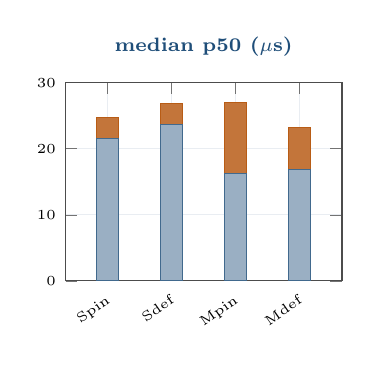
\begin{tikzpicture}
\begin{axis}[
  width=0.42\columnwidth, height=4.1cm,
  ybar stacked, bar width=8pt,
  symbolic x coords={Spin, Sdef, Mpin, Mdef},
  xtick=data, enlarge x limits=0.22, ymin=0, ymax=30,
  x tick label style={font=\tiny, rotate=35, anchor=north east},
  y tick label style={font=\tiny},
  title={median p50 ($\mu$s)},
  axis line style={black!70},
]
\addplot[fill=cblue!45, draw=cblue!85] coordinates
  {(Spin,21.6) (Sdef,23.7) (Mpin,16.2) (Mdef,16.8)};
\addplot[fill=corange!80, draw=corange!95] coordinates
  {(Spin,3.1) (Sdef,3.1) (Mpin,10.8) (Mdef,6.4)};
\end{axis}
\end{tikzpicture}%
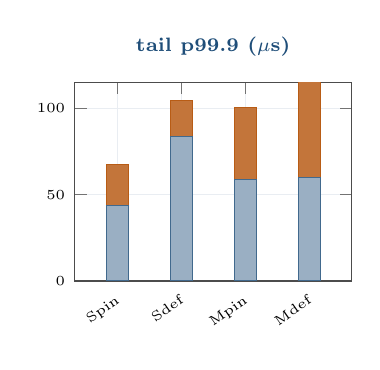
\begin{tikzpicture}
\begin{axis}[
  width=0.42\columnwidth, height=4.1cm,
  ybar stacked, bar width=8pt,
  symbolic x coords={Spin, Sdef, Mpin, Mdef},
  xtick=data, enlarge x limits=0.22, ymin=0, ymax=115,
  x tick label style={font=\tiny, rotate=35, anchor=north east},
  y tick label style={font=\tiny},
  title={tail p99.9 ($\mu$s)},
  axis line style={black!70},
]
\addplot[fill=cblue!45, draw=cblue!85] coordinates
  {(Spin,43.9) (Sdef,83.8) (Mpin,58.7) (Mdef,60.2)};
\addplot[fill=corange!80, draw=corange!95] coordinates
  {(Spin,23.6) (Sdef,20.7) (Mpin,42.0) (Mdef,102.6)};
\end{axis}
\end{tikzpicture}
\caption{Where the latency sits, at the median and at p99.9, for the four
queue/scheduler combinations with \texttt{epoll}: blue is arrival (send to
parse), orange is service (parse to done), and the tick labels are
S\,=\,$\texttt{SPSC}$, M\,=\,$\texttt{mutex}$, pin/default abbreviated.
Arrival dominates every median, so no amount of matching-engine optimization
could move the typical number. At p99.9 the mutex configurations buy a smaller
arrival component and pay for it with a $2$--$3.5\times$ larger service
component at the median and $1.8$--$5\times$ at p99.9. The two components are
percentiles of their own distributions, measured on different orders, so they do
not add exactly to the total p99.9 of Table~\ref{tab:latency}. Values from
Table~\ref{tab:decomposition}.}
\label{fig:split}
\end{figure}

The mutex rows invert part of the ratio. Their arrival component is \emph{lower}
in absolute terms (59--69\us) because a sleeping consumer leaves the network
thread undisturbed, but service rises to 42--103\us. Median over the four
configurations: service p99.9 is 20.7\us{} for SPSC and 68.6\us{} for mutex, a
factor of 3.3. The V1 row inverts the ratio completely: arrival is normal at
47\us, service is 6.50\,ms, and 99.7\% of the tail is inside the book.

\begin{table*}[!t]
\centering
\caption{Arrival (client send to parse) and service (parse to completion)
components, same runs as Table~\ref{tab:latency}. The total columns are dropped
because they are already there; what remains is the split. Latencies in
$\mu$s.}
\label{tab:decomposition}
\small
\setlength{\tabcolsep}{7pt}
\begin{tabular}{@{}lrrrrr@{}}
\arrayrulecolor{cblue}\toprule
\rowcolor{cblueL}\textbf{Configuration} &
  \multicolumn{2}{c}{\cellcolor{cblue!22}\textbf{arrival}} &
  \multicolumn{2}{c}{\cellcolor{corange!22}\textbf{service}} &
  \cellcolor{cgreen!22}\textbf{tail share} \\
\rowcolor{cblueL}\textbf{} & \textbf{p50} & \textbf{p99.9} & \textbf{p50} & \textbf{p99.9} & \textbf{arrival} \\
\arrayrulecolor{cblue!45}\midrule
SPSC / pinned / epoll     & 21.6 & 43.9 & 3.1 & 23.6 & 51\% \\
SPSC / pinned / io\_uring & 21.7 & 71.2 & 3.0 & 16.1 & 74\% \\
SPSC / default / epoll    & 23.7 & 83.8 & 3.1 & 20.7 & 66\% \\
SPSC / default / io\_uring& 21.2 & 86.4 & 3.1 & 27.1 & 71\% \\
\arrayrulecolor{corange!45}\midrule
mutex / pinned / epoll    & 16.2 & 58.7 & 10.8 & 42.0 & 56\% \\
mutex / pinned / io\_uring& 19.9 & 60.9 & 10.4 & 42.3 & 54\% \\
mutex / default / epoll   & 16.8 & 60.2 & 6.4 & \textcolor{cred}{\textbf{102.6}} & 38\% \\
mutex / default / io\_uring & 17.3 & 69.2 & 6.1 & 95.0 & 46\% \\
\arrayrulecolor{cgreen!45}\midrule
allocator: V1 book       & 21.1 & 47.3 & 2.7 & \textcolor{cred}{\textbf{6\,500}} & \textcolor{cred}{\textbf{1\%}} \\
\arrayrulecolor{cblue}\bottomrule
\end{tabular}
\end{table*}

\reading{Read the rightmost column first. When it is small, the tail is inside
the book or the queue; when it is 51--74\%, the tail is the network thread
failing to get a CPU.}

\subsection{Queue: Mutex Versus Lock-Free SPSC}
Holding the book, network and scheduling fixed, the queue comparison is
statistically resolvable at p99 and at the service tail, and not at the median
(Table~\ref{tab:queuetests}).

\begin{table}[!t]
\centering
\caption{Queue comparison on clean runs, two-sided exact permutation test on the
difference of medians. Green $p$ values are resolvable at $n=9$--10, grey ones
are not.}
\label{tab:queuetests}
\small
\setlength{\tabcolsep}{4pt}
\begin{tabular}{@{}llrrr@{}}
\arrayrulecolor{cblue}\toprule
\rowcolor{cblueL}\textbf{Percentile} & \textbf{Pair} & \textbf{SPSC} & \textbf{mutex} & \textbf{$p$} \\
\arrayrulecolor{cblue!45}\midrule
p50           & default/\texttt{epoll} & 26.8 & 24.3 & \textcolor{cgray}{0.145} \\
p99           & default/\texttt{epoll} & 38.9 & 71.7 & \textcolor{cgreen}{\textbf{0.0008}} \\
p99           & pinned/\texttt{epoll}  & 38.3 & 70.9 & \textcolor{cgreen}{\textbf{0.0015}} \\
service p99.9 & pinned/\texttt{epoll}  & 20.7 & 42.0 & \textcolor{cgreen}{\textbf{0.0008}} \\
total p99.9   & pinned/\texttt{epoll}  & 86.8 & 105.3 & \textcolor{cgray}{0.143} \\
\arrayrulecolor{cblue}\bottomrule
\end{tabular}
\end{table}

\textbf{Mechanism.} At the median the queues are the same because at
200\,000 orders/s the ring is almost never empty; both hand off in nanoseconds.
The difference appears where the consumer must wait. A condition variable parks
the consumer, so each batch costs a wakeup: the producer enters the kernel, a CPU
is chosen for the consumer, and the consumer resumes with a cold pipeline. That
cost appears as 157\,000--199\,000 voluntary switches in the \emph{producer} and
as a 102.6\us{} service tail---not as arrival tail, which is why the mutex rows
have a lower arrival share. The SPSC consumer never sleeps: it spins, observes
the published index within a few hundred nanoseconds, and proceeds. The
throughput rows confirm the same mechanism from the other direction: 5.29 versus
3.19\Mops{} and 0.19 versus 0.32\us{} of engine CPU per order. The SPSC buffer
does its own waiting instead of asking the kernel to do it.

\reading{The queue is not a median decision, it is a decision about who waits:
the kernel or the core.}

\subsection{Allocator}
In isolation, on 2\,000\,000 64-byte allocations with a live set of 8192, the
slab averages 12.59\ns{} per allocation and 14.13\ns{} per release, against
17.14\ns{} and 22.19\ns{} for aligned \texttt{operator new}/\texttt{delete}:
$1.36\times$ and $1.57\times$ faster, with standard deviations of 6.9 and 8.5\ns{}
against 27.5 and 86.2\ns. Both variants pay 20--25\ns{} of clock overhead, so the
ratio and the spread are the meaningful numbers.

End-to-end the difference is not resolvable. At 200\,000 orders/s on the same
pipeline, slab gives 98.7\us{} p99.9 and heap gives 119.5\us{} ($p=0.37$), with
run ranges of 57.7--147.5 and 67.9--150.5\us. Allocation is off the critical
path: the 25\us{} of ingress and wake-up covers it. A fixed-size allocation is
served from glibc's per-thread cache in tens of nanoseconds, and the slab's
advantage lives in the tail and the variance, where the component benchmark can
see it but the integrated harness cannot.

The V1 row is the real allocator lesson. Its service p99.9 is 6.50\,ms with a
run-to-run range of 6.14--7.05\,ms: reproducible, not an outlier. In the raw
per-order samples the slow orders form clusters of arbitrary size (431, 1046,
2738 orders) at arbitrary offsets, whereas host-delay clusters are built from
whole 64-order client batches---the signature of a book-side stall. The
mechanism is \texttt{std::unordered\_map} rehashing plus one heap node per
operation; the V3-with-heap control rules out \texttt{operator new} alone (same
allocator call, $55\times$ smaller p99.9), because the sizes are fixed and the
containers never rehash.

\subsection{Scheduling and Affinity}
Pinning the engine does not give it the core. Without \texttt{isolcpus} and
without realtime priority, ordinary work is still scheduled on CPU 2, and a
pinned thread cannot migrate away. The counters show exactly that, and they
behave differently for the two queue types.

With the spinning queue the engine is already runnable when work arrives, so its
accumulated run-queue wait is small: 2.20\,ms unpinned and 0.22\,ms pinned, a
tenfold reduction. With the blocking queue the engine is asleep between batches:
every wakeup is a new scheduling decision, and \texttt{schedstat} accumulates the
wait of $\sim$17\,000 voluntary sleeps, reaching 72.6\,ms (range 0.08--154\,ms)
in the pinned configuration while median latency stays at 27\us. That figure is
accumulated wake-up delay, not a stall, and reading it as a stall would be wrong.

Pinning improved p99.9 from 127.7\us{} to 85.6\us{}, a 33\% reduction that does
not reach significance at $n=10$ ($p=0.14$), because the network thread still
floats and it is the component that absorbs host interference. The expected
benefit requires \texttt{isolcpus} or a cpuset, which this host forbade, and the
\texttt{SCHED\_FIFO} arm failed with \texttt{EPERM}. The realtime experiment is
therefore a documented null result by host policy, not by design.

\subsection{Network Backend}
Latency and throughput are indistinguishable between \texttt{epoll} and
\texttt{io\_uring} (Table~\ref{tab:throughput}); the p99.9 ordering reverses
between the pinned and unpinned pairs, so no latency winner is claimed. What does
differ, and inverts with load, is the syscall count. At 200\,000 orders/s the
client sends 64-order batches every 320\us: \texttt{io\_uring} needs one submit
and one completion per batch (31.6k operations), while \texttt{epoll} needs one
wait plus at least one productive and one \texttt{EAGAIN} read (47.3k
operations), so \texttt{io\_uring} needs 33\% fewer. Unthrottled, the socket is
always non-empty: \texttt{epoll}'s drain loop amortises one wait over many reads
(20.2k operations for 2\,M orders), while \texttt{io\_uring} re-posts one
submission per read (40.3k), so \texttt{epoll} needs 50\% fewer. Fewer syscalls
is not the same as lower latency, and here it was not.

\subsection{Throughput and CPU Accounting}
Table~\ref{tab:throughput} and Fig.~\ref{fig:tp} give the unthrottled results.
SPSC reaches 5.86\Mops{} at 0.17\us{} of engine CPU per order; the mutex path
reaches 3.38\Mops{} at 0.30\us{} and pays 157\,000--199\,000 voluntary switches
for it. The network thread costs 0.17--0.21\us{} per order in every
configuration, which is the control that says the queue is what changed.

\begin{figure}[!t]
\centering
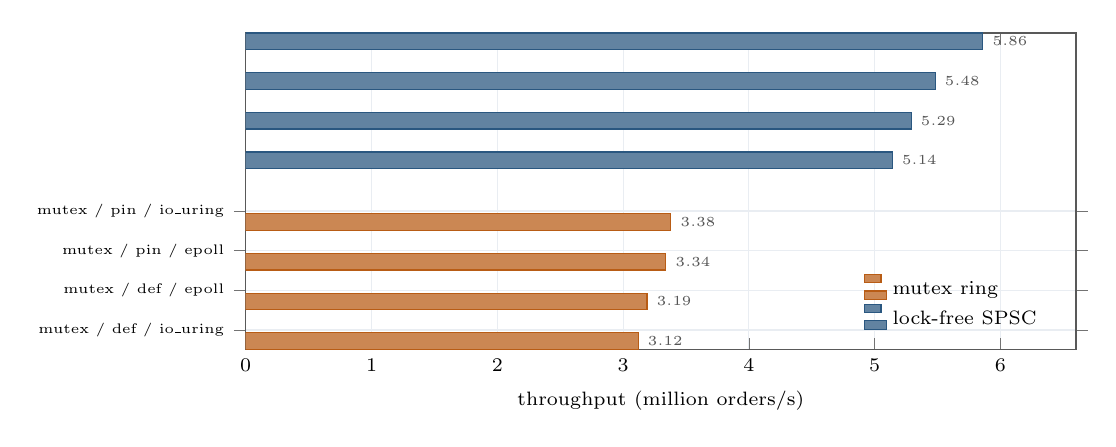
\begin{tikzpicture}
\begin{axis}[
  width=\columnwidth, height=5.6cm,
  xbar, xmin=0, xmax=6.6, bar width=6pt,
  symbolic y coords={mdu, mde, mpe, mpu, sdu, sde, spu, spp},
  ytick=data,
  yticklabels={mutex / def / io\_uring, mutex / def / epoll,
               mutex / pin / epoll, mutex / pin / io\_uring,
               SPSC / def / io\_uring, SPSC / def / epoll,
               SPSC / pin / io\_uring, SPSC / pin / epoll},
  y tick label style={font=\tiny},
  xlabel={throughput (million orders/s)},
  legend pos=south east, legend cell align=left,
  nodes near coords, nodes near coords style={font=\tiny, color=cgray},
  enlarge y limits=0.07,
]
\addplot[fill=corange!70, draw=corange!95] coordinates {
  (3.12,mdu) (3.19,mde) (3.34,mpe) (3.38,mpu)};
\addplot[fill=cblue!70, draw=cblue!95] coordinates {
  (5.14,sdu) (5.29,sde) (5.48,spu) (5.86,spp)};
\legend{mutex ring, lock-free SPSC}
\end{axis}
\end{tikzpicture}
\caption{Unthrottled throughput, same runs as Table~\ref{tab:throughput}. The
queues do not overlap: the slowest SPSC configuration beats the fastest mutex
one by $1.52\times$, and the best case is $1.75\times$. The SPSC bars are
client-limited (the generator cannot push past 5.9\Mops), so the server ceiling
is higher than the bar; the mutex bars are a genuine service limit.}
\label{fig:tp}
\end{figure}

These unthrottled SPSC figures are \emph{client-limited}: the client sends
1024-order batches, blocks on a full socket and delivers 5.5--5.9\Mops, so the
number is a harness limit rather than a server limit. Section~\ref{sec:sat}
shows the same pipeline absorbing 6.4\Mops{} with zero full-queue waits, so the
server ceiling is above 6.4\Mops. The mutex numbers, by contrast, are a genuine
service result.

The CPU columns are the clearest OS-level trade-off in the study. At
200\,000 orders/s the SPSC engine reports about 101\% of a core---one core fully
occupied, mostly spinning---while the mutex engine reports 8--9\% because it
sleeps. The lock-free queue buys tail latency and overload tolerance by keeping
a core busy.

\begin{table*}[!t]
\centering
\caption{Unthrottled runs (2\,M orders, 5 repetitions): engine CPU per order and
syscall accounting. Throughput itself is in Fig.~\ref{fig:tp}, so the columns
here are the ones the figure cannot show. CPU per order in $\mu$s.}
\label{tab:throughput}
\small
\setlength{\tabcolsep}{9pt}
\begin{tabular}{@{}lrrr@{}}
\arrayrulecolor{cblue}\toprule
\rowcolor{cblueL}\textbf{Configuration} & \textbf{engine CPU/order} & \textbf{network \texttt{nvcsw}} & \textbf{kernel ops/run} \\
\arrayrulecolor{cblue!45}\midrule
\rowcolor{cblueL!55}SPSC / pinned / epoll     & \textbf{0.17} & 12 & 20\,190 \\
\rowcolor{cblueL!55}SPSC / pinned / io\_uring & 0.18 & 12 & 40\,328 \\
\rowcolor{cblueL!55}SPSC / default / epoll    & 0.19 & 15 & 20\,194 \\
\rowcolor{cblueL!55}SPSC / default / io\_uring& 0.19 & 15 & 40\,328 \\
\arrayrulecolor{corange!45}\midrule
\rowcolor{corangeL!70}mutex / pinned / io\_uring& 0.30 & \textcolor{cred}{157\,151} & 40\,328 \\
\rowcolor{corangeL!70}mutex / pinned / epoll    & 0.30 & \textcolor{cred}{172\,731} & 20\,170 \\
\rowcolor{corangeL!70}mutex / default / epoll   & 0.32 & \textcolor{cred}{159\,756} & 20\,168 \\
\rowcolor{corangeL!70}mutex / default / io\_uring & \textbf{0.32} & \textcolor{cred}{198\,511} & 40\,328 \\
\arrayrulecolor{cblue}\bottomrule
\end{tabular}
\end{table*}

\reading{Five orders of magnitude separate the two columns that matter: the
lock-free path burns CPU time and saves context switches; the blocking path does
the reverse.}

\subsection{Saturation}
\label{sec:sat}
Table~\ref{tab:saturation} sweeps the offered rate and Fig.~\ref{fig:sat} plots
the same sweep. Four findings:

\begin{figure}[!t]
\centering
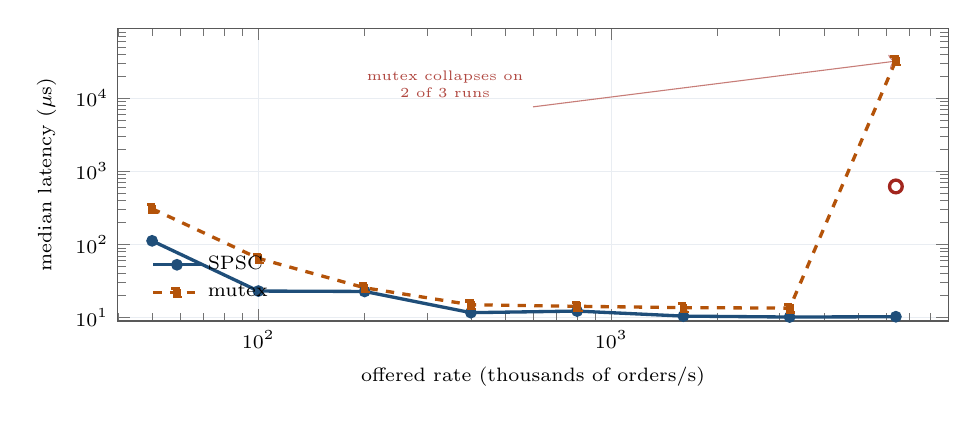
\begin{tikzpicture}
\begin{axis}[
  width=\columnwidth, height=5.3cm,
  xmode=log, ymode=log,
  xmin=40, xmax=9000, ymin=9, ymax=90000,
  xlabel={offered rate (thousands of orders/s)},
  ylabel={median latency ($\mu$s)},
  legend pos=south west, legend cell align=left,
]
\addplot[cblue, very thick, mark=*, mark size=1.5pt] coordinates {
  (50,112.1) (100,23.1) (200,22.8) (400,11.7)
  (800,12.3) (1600,10.5) (3200,10.2) (6400,10.3)};
\addplot[corange, very thick, dashed, mark=square*, mark size=1.4pt] coordinates {
  (50,308.0) (100,64.6) (200,25.6) (400,15.0)
  (800,14.3) (1600,13.7) (3200,13.5) (6400,32647)};
\addplot[only marks, mark=o, mark size=2.3pt, cred, very thick] coordinates {(6400,620)};
\legend{SPSC, mutex}
\node[font=\tiny, color=cred!85, align=center, anchor=north east] (a)
  at (axis cs:600,32000) {mutex collapses on\\2 of 3 runs};
\draw[->, cred!60, thin] (a.south east) -- (axis cs:6400,32000);
\end{axis}
\end{tikzpicture}
\caption{Median latency against offered rate, medians of three runs. Both
queues get \emph{faster} up to about 3.2\Mops{} because wake-up cost is
amortised over larger batches; below 200\,000 orders/s the blocking queue is
$2.7\times$ slower, which is the regime where it loses most. At 6.4\Mops{} the
SPSC path is unchanged; the mutex marker is the median of three runs, two of
which collapsed to a 32.7\,ms median, and the open circle is the single run that
survived at 0.62\,ms. Values from Table~\ref{tab:saturation}.}
\label{fig:sat}
\end{figure}

\textbf{The SPSC queue is not near saturation.} It returned 6.40\Mops{} in three
of three runs with zero full-queue waits; the harness cannot offer more. The cost
sits on the other side: 43\,158 of 3\,000\,000 pops (1.4\%) found the ring empty
and had to spin. At the unthrottled closed-loop rate the queue does fill
(1.84\,M full waits), because a 1024-order batch arrives faster than 64 bytes per
order can be matched; that row measures client-blocked response time, not queue
capacity.

\textbf{The mutex path is bistable, not capped.} Two of three runs at 6.4\Mops
collapsed to about 3.3\Mops{} with a 32.7\,ms median, 414\,000--495\,000 blocking
pushes and 208\,000--259\,000 voluntary switches in the network thread. The third
run kept up: 6.01\Mops{} at a 0.62\,ms median with 26\,654 full waits, but still
a 30.9\,ms worst case at the end of the run. With three repetitions this is a
warning rather than an estimate. The stable ceiling is 3.2\Mops{} (zero waits),
the collapse point is below 6.4\Mops, and whether a run collapses appears to
depend on which sleep/wake pattern the two threads settle into.

\textbf{Closed-loop throughput alone would hide this.} The unthrottled client
blocks on the socket, so the mutex pipeline settles at 3.3\Mops{} in three of
three runs; the open-loop sweep shows the same code reaching 6.0\Mops{} when it
happens not to collapse. The two measurements bound the behaviour; neither is
the whole answer.

\textbf{Latency is not monotonic in offered rate.} Both queues get faster as the
rate rises from 50\,k/s to about 3.2\Mops{} (mutex 308 to 13.5\us, SPSC 112 to
10.2\us) because wake-up cost is amortised over larger batches. Below
200\,k/s the blocking queue is $2.7\times$ slower at the median. The idle case is
where the mutex loses most, not the busy case: at low load every order pays a
full sleep and wake.

\begin{table}[!t]
\centering
\caption{Saturation sweep, medians of 3 runs. Offered rates in thousands of
orders/s; p50 in $\mu$s; full waits are blocking pushes. Achieved equalled
offered in every row except the collapse (3\,320) and the unthrottled runs
(5\,560 and 3\,330).}
\label{tab:saturation}
\small
\setlength{\tabcolsep}{4pt}
\begin{tabular}{@{}rrrrr@{}}
\arrayrulecolor{cblue}\toprule
\rowcolor{cblueL}\textbf{Offered} &
  \multicolumn{2}{c}{\cellcolor{cblue!22}\textbf{SPSC}} &
  \multicolumn{2}{c}{\cellcolor{corange!22}\textbf{mutex}} \\
\rowcolor{cblueL}\textbf{(k/s)} & \textbf{p50} & \textbf{full waits} &
  \textbf{p50} & \textbf{full waits} \\
\arrayrulecolor{cblue!45}\midrule
50     & 112.1 & 0 & 308.0 & 0 \\
100    & 23.1  & 0 & 64.6  & 0 \\
200    & 22.8  & 0 & 25.6  & 0 \\
400    & 11.7  & 0 & 15.0  & 0 \\
800    & 12.3  & 0 & 14.3  & 0 \\
1\,600 & 10.5  & 0 & 13.7  & 0 \\
3\,200 & \textbf{10.2} & 0 & \textbf{13.5} & 0 \\
\rowcolor{credL}\textbf{6\,400} & \textbf{10.3} & \textbf{0} &
  \textcolor{cred}{\textbf{32\,650}} & \textcolor{cred}{\textbf{414\,210}} \\
\rowcolor{credL}unthrottled & 12\,860 & 1\,841\,316 & 21\,480 & 249\,965 \\
\arrayrulecolor{cblue}\bottomrule
\end{tabular}
\end{table}

\reading{The lock-free queue has no knee in the measured range; the blocking
queue does, and it is a cliff rather than a ceiling: the same code either holds
6.0\Mops{} or loses half of it depending on which sleep pattern it settles
into.}

\subsection{False Sharing on the SPSC Boundary}
Two buffers with byte-identical push/pop logic differ only in layout:
\emph{padded} gives each ownership domain its own cache line (what the production
queue does), \emph{packed} puts all four indices adjacent~\cite{bolosky}. Over
5\,M orders per repetition and 9 repetitions, padded reaches a median
8.59\Mops{} (best 9.66) at 153\ns{} median latency, and packed reaches
10.28\Mops{} (best 11.78) at 197\ns.

The honest reading is a trade-off, not a win. Per-item latency favours padding
in 18 of 18 repetitions across two independently measured host conditions
(two-sided sign test, $p\approx 8\times10^{-6}$). Throughput moves the other way
in 8 of 9 repetitions here, but the contended repetition had padding ahead in 3
of 9, so the throughput direction is not stable and no throughput claim is made.
The plausible mechanism---not verified here---is that packing lets the slot write
and the index publish land on the same line, which reduces line transfers per
item (higher rate) while putting both threads on one line (higher per-item
latency). The production queue also caches the peer index locally, so the remote
line is touched only when the queue looks empty or full; this benchmark does not
exercise that path, so it cannot justify the production layout. Padding is kept
because the mechanism is sound and the alternative has no demonstrated advantage.

\subsection{Probes and Host Sensitivity}
Three probes bound the remaining explanations. With the client free to migrate,
p99.9 is 63.8\us{} against 51.5\us{} pinned, and no order is late, so client
pinning is a legitimate control rather than a way of hiding client jitter.
Pinning the network thread raises p99.9 from 51.5 to 127.5\us{} and the worst
arrival delay from 293 to 988\us, with 192 late orders in one of three runs: a
confined thread loses the ability to migrate away from unrelated work, the same
lesson as Section~\ref{sec:results} measured on the producer side.

The host itself was measured as a variable. Table~\ref{tab:host} reports the same
binary and configuration under three conditions. Confining the competing desktop
process to the E-cores moved p99.9 by a factor of 17 with no code change, while
the engine's own run-queue wait stayed at 0.29\,ms, so the engine was not the
delayed component. The per-run fingerprint is unambiguous: \texttt{net\_ingest\_slow}
in the thousands, network run-queue wait in the tens of milliseconds, arrival
p99.9 near 2.4\,ms and service p99.9 unchanged. Every ordering that matters
survives the change of host condition---SPSC over mutex on throughput
($1.58\times$ contended, $1.75\times$ quiet), V3 over V1 on the tail, slab over
heap in isolation, padding over packing on per-item latency---so the orderings
are properties of the code. What does not survive is the absolute tail, which is
a property of the machine.

The median, notably, is insensitive to contention: 22.6--33.0\us{} in the
contended condition and 23.8--29.1\us{} in the quiet one. Removing contention
does not make a wake-up cheaper; it removes the multi-millisecond delays that
dominate p99.9. Fig.~\ref{fig:host} is the clearest single result in the study:
the same binary, the same configuration, and a $17\times$ change in the tail
caused by what else is running on the machine.

\begin{figure}[!t]
\centering
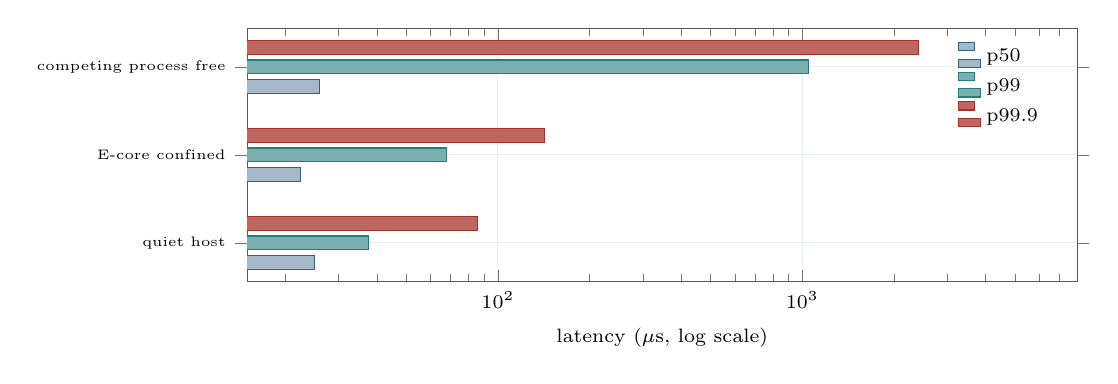
\begin{tikzpicture}
\begin{axis}[
  width=\columnwidth, height=4.8cm,
  xmode=log, xbar, xmin=15, xmax=8000, bar width=5pt,
  symbolic y coords={quiet, Ecore, contended},
  ytick=data,
  yticklabels={quiet host, E-core confined, competing process free},
  y tick label style={font=\tiny},
  xlabel={latency ($\mu$s, log scale)},
  legend pos=north east, legend cell align=left,
  enlarge y limits=0.22,
]
\addplot[fill=cblue!40, draw=cblue!90] coordinates {
  (25.0,quiet) (22.5,Ecore) (26.0,contended)};
\addplot[fill=cteal!55, draw=cteal!90] coordinates {
  (37.6,quiet) (68,Ecore) (1046,contended)};
\addplot[fill=cred!70, draw=cred!95] coordinates {
  (85.6,quiet) (142,Ecore) (2400,contended)};
\legend{p50, p99, p99.9}
\end{axis}
\end{tikzpicture}
\caption{Host sensitivity of one binary and one configuration
(SPSC / pinned / \texttt{epoll}), from Table~\ref{tab:host}. The medians barely
move between conditions; the p99.9 does. Confining an unrelated desktop process
to the E-cores took the tail from 2.40\,ms to 142\us{} without touching a line of
server code, and the run's own counters attribute the delay to the network
thread's run-queue wait (97.7\,ms against 1.2\,ms), not to the engine.}
\label{fig:host}
\end{figure}

\begin{table}[!t]
\centering
\caption{Host sensitivity, same binary and configuration
(SPSC / pinned / \texttt{epoll}). p99.9 in $\mu$s; late orders were already
$>$1\,ms old at parse.}
\label{tab:host}
\small
\setlength{\tabcolsep}{4pt}
\begin{tabular}{@{}lrrr@{}}
\arrayrulecolor{cblue}\toprule
\rowcolor{cblueL}\textbf{Condition} & \textbf{p99.9} & \textbf{net runq} & \textbf{orders $>$1\,ms} \\
\arrayrulecolor{cblue!45}\midrule
\rowcolor{credL}competing process free & \textcolor{cred}{\textbf{2\,400}} & 97.7\,ms & \textcolor{cred}{\textbf{10\,017}} \\
\rowcolor{cgreenL}competing process on E-cores & 142 & 1.2\,ms & \textbf{0} \\
\rowcolor{cblueL!60}quiet host, \texttt{performance} & \textbf{85.6} & 0.5\,ms & \textbf{0} \\
\arrayrulecolor{cblue}\bottomrule
\end{tabular}
\end{table}

\reading{A tail number is a statement about a machine at a moment, not about a
program. The only defensible absolute claim is the one qualified by the
condition it was measured in.}

\section{Discussion}
\label{sec:discussion}

\textbf{Where does latency go?} On loopback TCP it goes to ingress. The book
needs 0.094\us{} at the median and 0.374\us{} at p99.9; the queue adds about
0.2\us; the network path adds about 22\us{} at the median and 44--86\us{} at
p99.9. The pipeline without a network costs 0.299\us{} and 13.2\us. Any
optimization aimed at the matcher would have been invisible.

\textbf{Does synchronization matter?} Yes, where a thread must wait, and not at
the median. The SPSC ring halves p99, cuts the matching-side p99.9 by
$3.3\times$ and raises throughput $1.75\times$, because it replaces a kernel
wakeup with a spin; the four-orders-of-magnitude reduction in producer context
switches is the mechanism, not a correlate. It also changes the failure mode at
overload from bistable collapse with 33\,ms medians to absorbing everything
offered.

\textbf{Does the allocator matter?} Only when the allocation pattern is
irregular. A fixed-size \texttt{new} is as good as a slab here ($p=0.37$); in
isolation the slab is $1.36$--$1.57\times$ faster with a quarter of the variance.
The 6.5\,ms tail belongs to growing, pointer-chasing containers, and the
V3-with-heap control isolates that.

\textbf{Does affinity help?} Not without isolation. Pinning cut the engine's
run-queue wait tenfold but improved p99.9 by 33\% with $p=0.14$: a real mechanism
without a significant end-to-end effect, because the floating network thread
absorbs the interference. Pinning the network thread made the tail worse.

\textbf{Is \texttt{io\_uring} faster?} Not in latency or throughput here. Its
benefit is syscall count under bursty, reader-faster-than-writer traffic, and it
reverses under saturation.

\textbf{Were the project's goals met?} The goal was an instrumented engine in
which each OS mechanism could be isolated and explained. Every comparison is
single-variable, every conclusion has a counter behind it, and all
configurations are numerically identical. One goal is only partly met: the
scheduling arm cannot demonstrate the realtime benefit without
\texttt{isolcpus}, \texttt{SCHED\_FIFO} and a fixed governor, so it is reported
as a null result.

\section{Threats to Validity}

\begin{itemize}
\item \emph{One host, one kernel, one compiler.} Every number is conditional on
this laptop's P/E-core topology. Ratios are more portable than absolutes.
\item \emph{Frequency is not fixed.} \texttt{powersave} leaves the governor in
charge; clocks held 4.2--4.4\,GHz during runs but idle at 0.8\,GHz between them.
$\pm$5\% throughput variance is consistent with this.
\item \emph{SMT is on.} The engine shares a physical core with its sibling; a
neighbour there would roughly halve its throughput. Not controlled, not observed.
\item \emph{No PMU counters.} \texttt{perf} was unavailable, so cache and branch
behaviour is absent; mechanism claims rest on in-process counters and A/B
controls.
\item \emph{Loopback only.} There is no NIC, no interrupt affinity and no kernel
bypass, so the arrival component would differ on real hardware, probably upward.
\item \emph{Client-limited throughput.} The unthrottled client cannot drive the
SPSC path past 5.9\Mops, so 6.4\Mops{} is a lower bound on the server ceiling.
\item \emph{Small $n$ at saturation.} Three repetitions cannot characterise a
bistable system; the collapse probability is unknown.
\item \emph{Arrival includes client work.} The generator stamps a batch after its
pacing wait but before building the 64 messages and calling \texttt{send}, so
arrival contains a few microseconds of client work and is quantised to batch
boundaries. This affects arrival, not service, and cannot reverse the
attribution.
\end{itemize}

\section{Related Work}

The bounded single-producer/single-consumer buffer and its correctness argument
are classical~\cite{lamport}; lock-free queue algorithms in general, and the
distinction between blocking and non-blocking progress guarantees, are treated by
Michael and Scott~\cite{michael} and by Herlihy and Shavit~\cite{herlihy}. The
C++ memory model that makes the \texttt{release}/\texttt{acquire} publication in
our ring buffer well defined is specified by Boehm and Adve~\cite{boehm}. False
sharing and its cost were characterised early by Bolosky and
Scott~\cite{bolosky}, and the cache-line-level reasoning behind the padded layout
follows their treatment.

On the I/O side, \texttt{io\_uring} was introduced as a completion-based
interface that amortises submission cost~\cite{axboe}; our measurement is a
concrete case in which that amortisation helps only when the reader is faster
than the writer. Methodologically we follow the systems-performance tradition of
measuring distributions rather than means and of separating queueing delay from
service time~\cite{gregg}, and we rely on the same memory-hierarchy facts
summarised by Drepper~\cite{drepper}.

\section{Conclusion}

The project set out to change one OS mechanism at a time and explain the latency
distribution. It did, and the explanation is less flattering to the
optimizations than expected. The matching engine is about 94\ns{} of work in a
pipeline whose p99.9 is about 87\us; 51--74\% of that tail is TCP ingress and
thread scheduling, and 86--88\% of the median is ingress and wake-up. The
lock-free queue earns its place in the tail, in throughput and in overload
behaviour rather than at the median: it absorbs 6.4\Mops{} that the mutex path
can lose to a 33\,ms median, at the cost of a permanently busy core. The slab
allocator is worst-case insurance; the dramatic tail belongs to the naive book,
not to \texttt{malloc}. Affinity and \texttt{io\_uring} did not measurably help,
and pinning without isolation moved a counter without moving the distribution.
The host is a variable of the same order as the code: a controlled confinement
experiment moves p99.9 from 2.4\,ms to 142\us{} with no code change.

The most useful artifact is therefore not the fastest configuration but the
ability to say, for any given run, which stage consumed the tail---with a counter
that proves it.

\begin{thebibliography}{9}

\bibitem{lamport}
L.~Lamport, ``Specifying concurrent program modules,'' \emph{ACM Trans. Program.
Lang. Syst.}, vol.~5, no.~2, pp.~190--222, Apr. 1983.

\bibitem{michael}
M.~M. Michael and M.~L. Scott, ``Simple, fast, and practical non-blocking and
blocking concurrent queue algorithms,'' in \emph{Proc. 15th ACM Symp. Principles
of Distributed Computing (PODC)}, 1996.

\bibitem{herlihy}
M.~Herlihy and N.~Shavit, \emph{The Art of Multiprocessor Programming}. San
Francisco, CA, USA: Morgan Kaufmann, 2008.

\bibitem{boehm}
H.-J. Boehm and S.~V. Adve, ``Foundations of the C++ concurrency memory model,''
in \emph{Proc. ACM SIGPLAN Conf. Programming Language Design and Implementation
(PLDI)}, 2008.

\bibitem{bolosky}
W.~J. Bolosky and M.~L. Scott, ``False sharing and its effect on shared memory
performance,'' in \emph{Proc. USENIX Symp. Experiences with Distributed and
Multiprocessor Systems (SEDMS)}, 1993.

\bibitem{axboe}
J.~Axboe, ``Efficient IO with io\_uring,'' 2019. [Online].
Available: \url{https://kernel.dk/io_uring.pdf}

\bibitem{gregg}
B.~Gregg, \emph{Systems Performance: Enterprise and the Cloud}, 2nd~ed. Boston,
MA, USA: Addison-Wesley, 2020.

\bibitem{drepper}
U.~Drepper, ``What every programmer should know about memory,'' Red Hat, Inc.,
Tech. Rep., 2007.

\end{thebibliography}

\end{document}
